\section{Dataset: MITBIH ECG data}
\begin{frame}{Heartbeat Arrhythmia}
    \begin{figure}
        \centering
        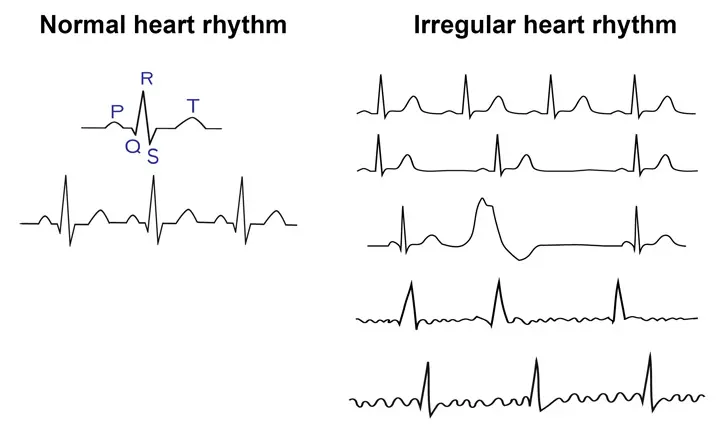
\includegraphics[scale=0.3]{images/heartbeat_arr.png}
        \caption[]{Different heartbeat arrhythmias \footnote{source: https://www.parkwayshenton.com.sg/health-plus/article/arrhythmia-guide}}
        \label{fig:enter-label}
    \end{figure}
\end{frame}

\begin{frame}{Arrhythmia Detection as an Anomaly Detection Problem}
We treat the problem of detecting anomalous heartbeats as an anomaly detection problem from machine learning based on the \alert{reconstruction error}:
\begin{itemize}
    \item<2->  We train a model \alert{on regular heartbeats} that is able to reconstruct that regular heartbeat.
    \item<3->  Given an anomalous heartbeat the model should give \alert{higher reconstruction error}.
    \item<4->  Based on an optimal \alert{threshold} for that error we classify this heartbeat as either regular or anomalous.
\end{itemize}
    \onslide<5>{Two reasons for this semi-supervised approach: high class imbalancy and no need for labelling.}
\end{frame} 

\begin{frame}{Baseline Model}
    Model is a LSTM-AE that is \alert{trained only on regular, private samples} with the goal to reconstruct normal samples. The classification is made based on the reconstruction error.
    \begin{columns}
        \begin{column}{0.48\textwidth}
        \begin{figure}
            \centering
            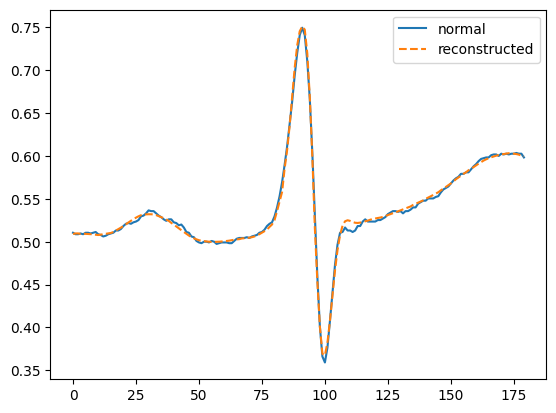
\includegraphics[scale=0.3]{images/rec_normal.png}
            \caption{reconstruction on normal sample \phantom{asdfsadf}}
            \label{fig:enter-label}
        \end{figure}
    \end{column}
    \begin{column}{0.48\textwidth}
        \begin{figure}
            \centering
            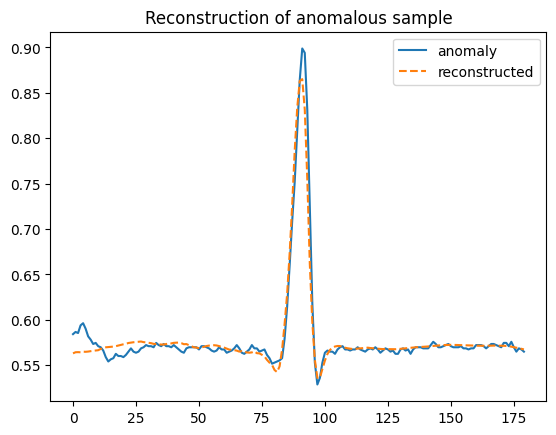
\includegraphics[scale=0.3]{images/rec_anom.png}
            \caption{reconstruction on anomalous sample}
            \label{fig:enter-label}
        \end{figure}
    \end{column}
    \end{columns}
\end{frame}

\begin{frame}
    \frametitle{Classification based on Reconstruction Error}

    \begin{columns}
        \begin{column}{0.48\textwidth}
        \begin{figure}
            \centering
            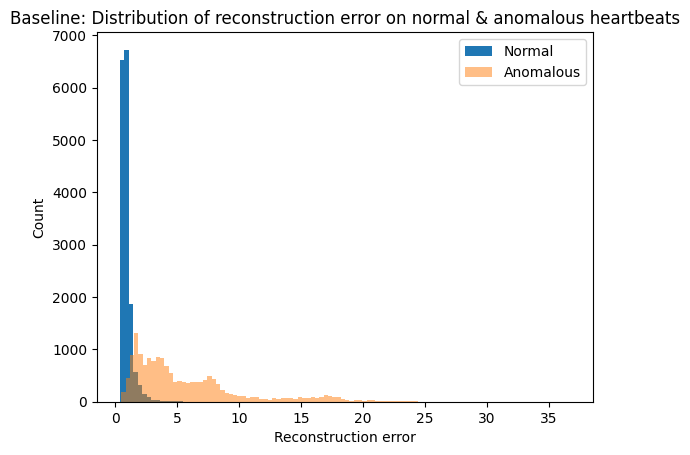
\includegraphics[scale=0.3]{hist_threshold_baseline.png}
            \caption{Distribution of reconstruction error on regular \& anomalous samples}
        \end{figure}
    \end{column}
    \begin{column}{0.48\textwidth}
        We can clearly see a \alert{difference in error distribution} for regular and anomalous samples. We choose the \alert{threshold that maximises the classification} accuracy.
    \end{column}
    \end{columns}

\end{frame}